% Created 2024-02-12 Mon 16:38
% Intended LaTeX compiler: pdflatex
\documentclass[presentation]{beamer}
\usepackage[utf8]{inputenc}
\usepackage[T1]{fontenc}
\usepackage{graphicx}
\usepackage{longtable}
\usepackage{wrapfig}
\usepackage{rotating}
\usepackage[normalem]{ulem}
\usepackage{amsmath}
\usepackage{amssymb}
\usepackage{capt-of}
\usepackage{hyperref}
\mode<beamer>{\usetheme{Madrid}}
\definecolor{SUred}{rgb}{0.59375, 0, 0.17969} % SU red (primary)
\definecolor{SUblue}{rgb}{0, 0.17578, 0.38281} % SU blue (secondary)
\setbeamercolor{palette primary}{bg=SUred,fg=white}
\setbeamercolor{palette secondary}{bg=SUblue,fg=white}
\setbeamercolor{palette tertiary}{bg=SUblue,fg=white}
\setbeamercolor{palette quaternary}{bg=SUblue,fg=white}
\setbeamercolor{structure}{fg=SUblue} % itemize, enumerate, etc
\setbeamercolor{section in toc}{fg=SUblue} % TOC sections
% Override palette coloring with secondary
\setbeamercolor{subsection in head/foot}{bg=SUblue,fg=white}
\setbeamercolor{date in head/foot}{bg=SUblue,fg=white}
\institute[SU]{Shenandoah University}
\titlegraphic{
\includegraphics[width=0.5\textwidth]{\string~/Documents/suLogo/suLogo.pdf}}
\newcommand{\R}{\mathbb{R}}
\usepackage{tikz}
\usepackage{pgfplots}
\usetheme{default}
\author{Chase Mathison\thanks{cmathiso@su.edu}}
\date{13 February 2024}
\title{Cylindrical Shells}
\hypersetup{
 pdfauthor={Chase Mathison},
 pdftitle={Cylindrical Shells},
 pdfkeywords={},
 pdfsubject={},
 pdfcreator={Emacs 29.1 (Org mode 9.6.7)}, 
 pdflang={English}}
\begin{document}

\maketitle

\section{Announcements}
\label{sec:orgde7ffd7}
\begin{frame}[label={sec:org64021e1}]{Announcements}
\begin{enumerate}
\item Exam Thursday (Pratice in MyOpenMath)
\item Office hours today 10am - 11am
\end{enumerate}
\end{frame}

\section{Lecture}
\label{sec:orgb89f0bb}
\begin{frame}[label={sec:orgf40841e}]{Last time}
Last time we talked about the washer method to find volumes of
revolution.

The disk method and the washer method are very powerful for finding
these volumes, but they still don't allow us to find some types of
volumes of revolution.

For example, let's try to find the volume of the solid that is
generated by rotating the region bounded by the graph of \(f \left( x
\right) = x - x^2\) and \(y = 0\) about the \(y-\)axis.
\end{frame}

\begin{frame}[label={sec:org53c6838}]{Example}
\end{frame}

\begin{frame}[label={sec:orgff50318}]{Cylindrical shells}
Clearly, trying to do this with the washer method is pretty awful.

It would be nice if we had an easier way to find the volume of
revolution when the region is defined in terms of functions of \(x\)
but rotated about the \(y-\)axis.

Enter: \uline{\hspace*{1in}}.

Let's illustrate the method of cylindrical shells on that last example
before we write down the general method.
\end{frame}

\begin{frame}[label={sec:org7b44d2e}]{Example}
Find the volume of the solid that is generated by rotating the region
bounded by the graph of \(f \left( x \right) = x - x^2\) and \(y = 0\) about the \(y-\)axis.

\begin{center}
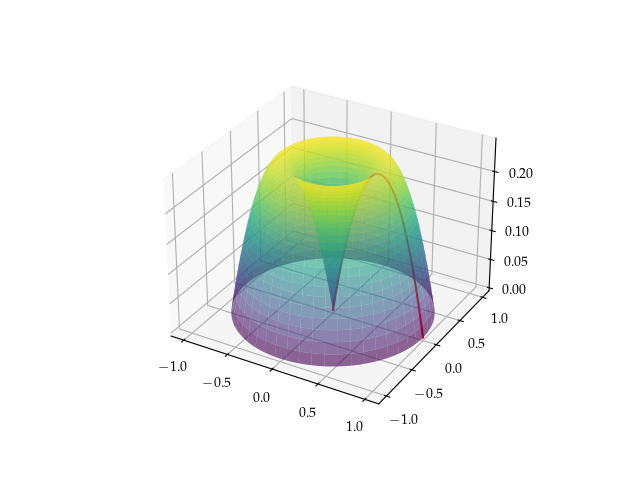
\includegraphics[width=0.5\textwidth]{../img/day008-ex01.png}
\end{center}
\vspace{10in}
\end{frame}

\begin{frame}[label={sec:orgdfb0a1b}]{Example}
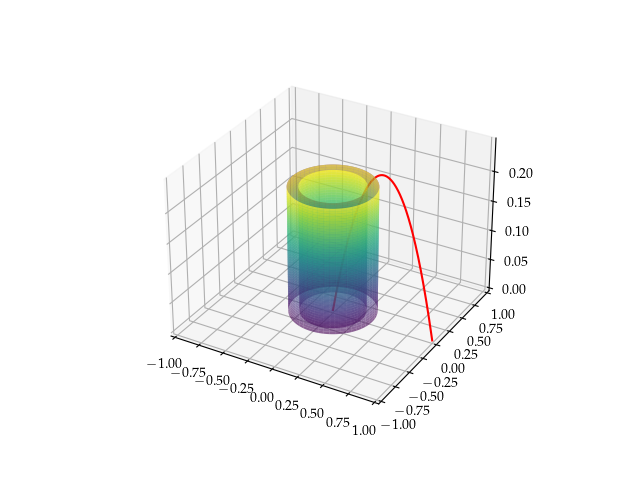
\includegraphics[width=0.5\textwidth]{../img/day008-ex02.png}
\vspace{10in}
\end{frame}


\begin{frame}[label={sec:org71ff232}]{Cylindrical shells, the general method}
What we did in the last example is exactly how we should proceed with
all cylindrical shell method problems.
\begin{theorem}[Cylindrical shell method]
Let \(f \left( x \right)\) and \(g \left( x \right)\) be continuous
and nonnegative with \(f \left( x \right) \ge g \left( x \right)\) on
the interval \(\left[ a,b \right]\).  Define \(R\) as the region
bounded above by the graph of \(f \left( x \right)\), below by the
graph of \(g \left( x \right)\) and by the lines \(x=a\) and \(x=b\). Then the volume of the solid generated by rotating \(R\) about the
\(y-\)axis is given by
\[
 \]
 \phantom{butts}

\phantom{butts}
\end{theorem}
\end{frame}

\begin{frame}[label={sec:org2ce0d50}]{Example}
Find the volume of the solid generated by rotating the region bounded
above by the graph of \(f \left( x \right) = \frac{e^x-1}{x}\), with
\(f \left( 0 \right) = 1\), below by \(y = 0\), and by the lines \(x
= 0\) and \(x = 2\) around the \(y-\)axis.

\begin{center}
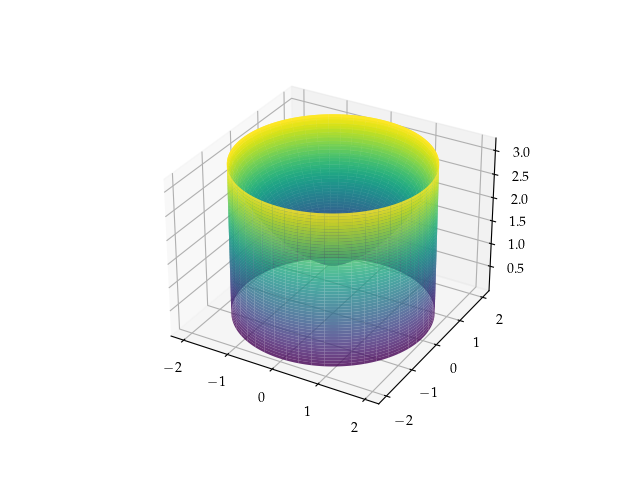
\includegraphics[width=0.5\textwidth]{../img/day008-ex03.png}
\end{center}
\end{frame}

\begin{frame}[label={sec:orgde2ff55}]{Example}
\end{frame}

\begin{frame}[label={sec:orgc53ae29}]{Cylindrical shells (functions of \(y\))}
Just like with the other methods, this easily generalizes to functions
of \(y\), with appropriate changes.
\begin{theorem}[Cylindrical shell method (for functions of \(y\))]
Let \(f \left( y \right)\) and \(g \left( y \right)\) be continuous
and nonnegative with \(f \left( y \right) \ge g \left( y \right)\) on
the interval \(\left[ c,d \right]\).  Define \(Q\) as the region
bounded on the right by the graph of \(f \left( y \right)\), on the left by the
graph of \(g \left( y \right)\) and by the lines \(y=c\) and \(y=d\). Then the volume of the solid generated by rotating \(Q\) about the
\(x-\)axis is given by
\[
 \]
 \phantom{butts}

\phantom{butts}
\end{theorem}
\end{frame}


\begin{frame}[label={sec:org0703e5d}]{Example}
Find the volume of the solid generated by rotating the region bounded
by the curves \(y = \sqrt{\ln \left( x \right)}\), \(y = 0\), and \(x = e^2\) about the \(x-\)axis.

\begin{center}
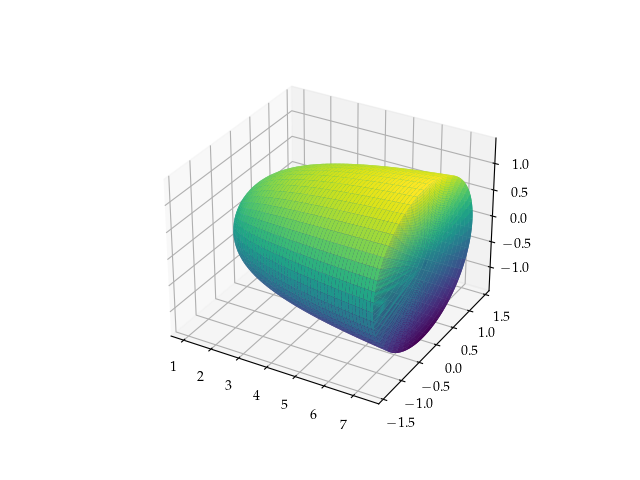
\includegraphics[width=0.5\textwidth]{../img/day008-ex04.png}
\end{center}
\vspace{10in}
\end{frame}

\begin{frame}[label={sec:org8527eec}]{Example}
\end{frame}


\begin{frame}[label={sec:orgb479809}]{So which method should I use?}
At this point you may ask, which method is the best one to use?  
The method you use depends heavily on the context of the problem.  For
instance, in the last example, we took a region defined in terms of a
function of \(x\) and rotated it about the \(x-\)axis, something
that usually we would use the disk or washer method for. 

But the disk method gave us an integral that we (currently) don't know
how to evaluate.  So in this case, we tried the cylindrical shell
method as a last ditch effort, and it happened to work out for us.

As a \emph{rule of thumb}, if you are rotating a region that is defined in
terms of functions of \(x\) about the \(x-\)axis, you'll
\uline{\hspace*{1in}} use the \uline{\hspace*{1in}} method.  If you are
rotating a region defined in terms of functions of \(x\) about the
\(y-\)axis, you'll \uline{\hspace*{1in}} use the \uline{\hspace*{1in}}.

Similar statements hold for functions of \(y\).
\end{frame}

\begin{frame}[label={sec:orge37fcac}]{Example}
Find the volume of the solid generated by rotating the region bounded
by the graphs of \(y = \left( e^x + e^{-x} \right)/2\), \(y = 0\)
and \(x = 1\), \(x = -1\) about the \(x-\)axis.
\vspace{10in}
\end{frame}

\begin{frame}[label={sec:org02620b0}]{Example}
\end{frame}

\begin{frame}[label={sec:org6409873}]{Example}
Find the volume of the solid generated by rotating the region bounded
by the curves \(y = x\), \(y = 2-x\) and \(y = 0\) about the \(x-\)axis.
\vspace{10in}
\end{frame}

\begin{frame}[label={sec:orgddc9d00}]{Example}
\end{frame}
\end{document}